
\part{Hybridity}
\section{Why Hybrid}

Virtually all optical phenomena can be modelled using ray tracing. The same can not be said for rasterization. 

\paragraph A typical problem with rasterization is the blending order of fragments needed for translucent surfaces. This is required if a scene contains more than one planar glass surface or any curved glass. Blending order can be solved using an A-buffer \cite{carpenter_1984} at the cost program complexity and memory. 

\paragraph Shadows using shadow maps have many problems. Ray tracing dosn't suffer aliasing to the same extent.

\paragraph Reflections must be done by rendering the scene seen from the surface that is to recieve reflections. Usually the scene is rendered into a cube map using six cameras. This is a crude approximation. Creating multiple reflection bounces quickly becomes more expensive. All surfaces visible in the reflection must be rendered multiple times. A ray tracer in comparison only needs traverse the rays affected.

\paragraph Refractions. Are done in the same manner as reflections.

So, will we in the future, once computational power is good enough to raytrace at retinal display quality only use ray tracing? Probably not. We surround ourselves with objects that have essentially only have diffuse shading. Glass house and porcelain shops are the exception, and even in such scenes, there are an abundance of diffuse surfaces.

Raytracing is essential for reflections. Just look at this car:

\begin{figure}[ht]
	\centering
	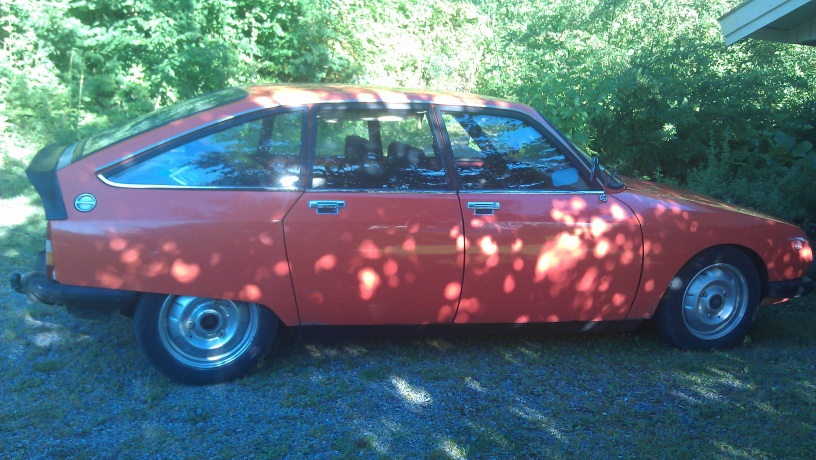
\includegraphics[width=0.80\textwidth]{Media/why_hybrid_carphoto.jpg}
	\caption{The car paint, glass and chrome details are essentially the only reflective surfaces in the scene}
	\label{fig:citroen_gs}
\end{figure}

\paragraph{Fill(rate) workload}
With rasterization, we often tell the GPU to shade large surfaces that out of view, the GPU quickly clips and discards fragments out side the view frustum. Pixar, as mentioned earlier solves this by cutting the geometry until it fits.

Ray tracing doesn't have this problem. We only try to shade what is visible.

\paragraph
Because of art pipelines and for the sake of simplicity, triangle based pipelines are the most popular.

A raytracer can be beneficial to render surfaces can naturally be intersected in an analytic raytracer or sampled by a discrete ray marcher.

Some examples are
\begin{itemize}
	\item Distance Fields can be raymarched, or an iso value can be extracted by solving the fields equation in an analytic raytracer. A rasterizer must usually sample all of the         field inside the view volume. This becomes especially problematic if the field changes on a frame-by-frame basis.

	\item Scalar Volume Data
	\item Spline surfaces
  \item Perfect analytical surfaces
\end{itemize}


% Unless a way to produce high bandwith memory, thats on par with CPU Registers, ray tracing will allways be slower.